\documentclass[12pt,a4paper]{report}
\usepackage{graphicx}
\usepackage[margin=1in]{geometry}
\usepackage{blindtext}
\usepackage[utf8]{inputenc}
\usepackage{array}
\usepackage{tikz}
\usetikzlibrary{positioning}
\usetikzlibrary{calc}
%\usetikzlibrary{shapes.geometry,arrows}
\usetikzlibrary{arrows,decorations.markings}
\usepackage{tikz-cd}
\usepackage{amsmath, amssymb}
%\usepackage[table]{xcolor}
\author{\Large \textit{SHATRUANJAY}}
\title{\Huge \textit{\textit{Index}}}
\date{\today}
\begin{document}
\maketitle
\tableofcontents{}
\chapter{Synopsis}
\newpage
\section{Project Title}
Host Intrusion Detection System for log files
\section{Project Option}
Internal Project
\section{Internal Guide}
Sushma A Shirke
\section{Technical Keywords}
\begin{enumerate}
\item	IDS \item	IPS \item	Firewall \item  Honeypot \item DDoS \item	Anomaly	\item	Shell	\item	NID	\item HID
\end{enumerate}

\section{Problem Statement}
We propose to build and demonstrate a novel system for rapid development and deployment of effective and cost-sensitive HIDSs. We consider intrusion detection as a classification problem, that is, we wish to classify each audit record or log records into one of a discrete set of possible categories, normal or a particular kind of intrusion. However, before we can apply classification algorithms, we need to first select and construct the right set of system features that may contain evidence (indicators) of normal or intrusions. We will develop an automatic feature selection and construction system to systematically discover and construct predictive features that can be used to build effective misuse and anomaly detection models. 
\newpage
\section{Abstract}
After the great revolution in the field of Information Technology, many applications made necessity to run computer systems (either servers or client machines) all the time. Along with improvements and new inventions in technology, the threat of attacks through computer networks becomes a large issue. Host Based Intrusion Detection is a part of security system that protects hosts from various kinds of attacks. It also provides a great degree of visibility (of system activities). It is quite widest that HIDS are vulnerable to attacks. An adversary, if successfully enters in a system can disable HIDS or modify HIDS rules to hide its existence. One can easily evade HIDS.We propose a new architecture that protects HIDS from such attacks. In this paper, we have proposed a new mechanism to check integrity of log files. We have discussed its affects on performance of system. 

\section{Goal And Objective}
The purpose of host intrusion detection's systems (HIDSs) is to monitor host systems with the express purpose of identifying and responding to suspicious activity.
\section{Names of conferences / journals where papers can be published}
\begin{itemize}
\item IEEE/ACM Conference/Journal 1
\item Conferences/workshops in IITs
\item Central Universities or SPPU Conferences
\item IEEE/ACM Conference/Journal 2
\end{itemize}

\newpage
\chapter{Technical Keywords}
\newpage
\section{Technical Keywords}
\begin{enumerate}
\item	IDS\\
\item	IPS\\
\item	Honeypot\\
\item	DDoS\\
\item	Anomaly\\
\item	Network based Intrusion Detection\\
\item	Host based Intrusion Detection\\
\item	Port Scanning \\
\item	TCP\\
\item	Attacks\\
\item	Snort\\
\item	Trojans\\
\item	Logs\\
\item	Client and Server\\
\item	IP Address\\
\item	Port and socket\\
\item	HTTP , SYN , UDP\\
\item	Ping\\

\end{enumerate}

\newpage
\chapter{Introduction}
\newpage
\section{Project Idea}
Our project is about making a host based intrusion detection system which is compatible with any traditional security system. We just need to set up a system and then we can easily work on the host and the network. We want our project to be based on open source tools and no proprietary software.
\section{Motivation Of The Project}
We referred several IEEE papers during the
initial stages of our project. 'An Effective Log Mining
Approach for Database Intrusion Detection'
published with IEEE paper standards describes that
due to sudden proliferation of networked applications,
database centered applications are facing a
rapidly growing number of threats. Malicious outsiders
launch attacks to access or corrupt data by
stealing access control credentials or exploiting application
vulnerabilities. On the Server side, server
admin may sabotage databases by abusing privileges.
Although various intrusion prevention and
detection mechanisms are employed to protect
against outsider and insider attacks, they are not
very effective in detecting attacks targeted on the
database at the server-side. The above mentioned
paper exhibits a novel scheme for identifying malicious
transaction patterns to detect attacks launched
either by outsiders or insiders on server database.

The IEEE paper titled 'Development of Host
Based Intrusion Detection System for Log Files' published with IEEE paper standards describes host
based intrusion describes host based intrusion detection
by using pattern matching technique on log
files. The system will recognize two types of attack
and its pattern. If an attack is unknown pattern, the
system needs to keep that pattern in the database for
the future assessment. Then, if an attack knows pattern,
the system will match that pattern in their database
and alert the host user about the attack or intrusion.
\begin{itemize}
\item Most Common Attacks (source CSI/FBI)
        In year 2014 most common attacks were:
        \begin{itemize}
        \item Virus (approx. 78\%)
\item Insider Abuse of Net Access (approx. 78\%)
\item Laptop theft (55\%)
\item Denial of Service and System Penetration (approx. 40\%)	
\item Unauthorized Access by Insiders (approx. 38\%)
        \end{itemize}

\item Developing absolutely secure systems is not possible
\begin{itemize}
\item Most existing systems have security flaws
\item	Abuses by privileged insiders are possible
\item Not all kinds of intrusions are known
\end{itemize}

\item Quick detection of intrusions can help to identify intruders and limit damage
\item IDS serves as a deterrent

\end{itemize}
\section{Literature Survey}
The aim of [1] is to address the issues of information security and describes the security needs of an organization to protect their critical information from attacks. A well trained staff and analysts are required to continuously monitor the system. But still a huge effort is required to construct new security strategies in this system which are discussed in [2], [9]. [2] Provides a multi-layer approach in IDPS to monitor a single host. Multi-layer approach consists of three layers. File Analyzer, System Resource Analyzer and Connection Analyzer. The advantage of this technique [2] is that it provides both signatures based and anomaly based detection and prevention. The drawback in Multi-layer approach is that the IDPS require a large amount of memory to store the data of the system and network traffic. 
Proventil desktop is software based solution [3] which detects and protects the system from network layer up to application layer by known and unknown attacks. This software has great flexibility to set 
different type of filtering rules. The major drawback of HIPS is its high rate of false-positives. A lot of time and trained staff is required to monitor the IDPS [3]. The idea discussed in [4] helps an organization to take an informal decision in order to select the IDPS. The proposed model divides the IDPS into two types,in-source and out-source. Provide a security to an organization against attacks is a key business of Managed Security Services Provider (MSSP) [4]. MSSP spend most of the time to examine new technology to secure the information better than before. A risk is possible if MSSP do not exactly know the customer requirements of IDPS. According to [5], Snort and source fire are best IPSs for a multinational company. Snort [5] product provides high flexibility that allow to the user to self-configure and modify its source code by using source fire. The major drawback of Snort is that it uses only signature based technique to detect the intrusion but if anomaly behavior occur then it will not be possible for SNORT to detect that anomaly attack [5]. Harley [8] defines the difference between host based and network based intrusion detection and prevention system. This paper describes two types of network intrusion detection system: Promiscuous-mode and Network-node. The main disadvantage observed is that this IDS only responds to the signature based detected attacks but not to the anomaly based detected attacks. So still there is a need of human interaction who took real time action to resolve issue [8]. 
Novel string matching technique [9] is an optimization of other matching algorithms. Novel string matching algorithm breaks the string into small sets of state machines. Each state machine recognizes the subset of string. If any suspicious behavior occurs then the system broadcasts the information about intruder to every module (state machine) which holds the data base in order to define rules and compares the signatures of intruder with predefined detected signatures. This algorithm is most efficient and ten times faster than the other existing systems and it consumes less resources. The major issue is its practical implementation and it requires a large amount of memory. This algorithm is not capable to detect the anomaly behavior of the intrusion as in [7].
According to S. Mrdovi and E. Zajko [10], Distributed IDS is used to analyze the system in which multiple sensors are placed in selected network segments that observe the network traffic behavior. SNORT is used as an analysis engine. MySQL is used to log the events with the help of SNORT. Distributed IDS is managed by management console which monitors and configures the IDS. This IDS provides a greater protection against attacks because multiple computers are continuously monitoring and preventing the network from malicious attacks [7]. Large memory and well trained security analysts are required to implement and continuous management of the system [7].
This paper [11] describes the security of IDS. It highlights the two different techniques of IDS. Misuse detection and anomaly detection. Three different approaches data mining, data fusion and immunological based approach used in IDS. This paper provides brief information about existing intrusion detection technology. It evaluates the challenges and future directions of intrusion detection technology. The approaches that are discussed in [4], [9] are much sufficient for IDPS to detect and respond to anomalies in real time. This paper [10] proposed intrusion detection techniques by combining multiple hosts in order to detect multiple intrusions and to reduce false-positive rate. Hidden Markov Model (HMM) is a speech recognition technique that is used for modeling the system call events. Statistical technique gives the percentage of resource usages and system call events. Decision tree is used to model or classify the type intrusion to examine the future challenges. This technique [10] has advantage of less false-positive rate that increases performance of detection. 
\newpage
\chapter{Problem Definition And Scope}
\newpage
\section{Problem Statement}
We propose to build and demonstrate a novel system for rapid development and deployment of effective and cost-sensitive HIDSs. We consider intrusion detection as a classification problem, that is, we wish to classify each audit record or log records into one of a discrete set of possible categories, normal or a particular kind of intrusion. However, before we can apply classification algorithms, we need to first select and construct the right set of system features that may contain evidence (indicators) of normal or intrusions. We will develop an automatic feature selection and construction system to systematically discover and construct predictive features that can be used to build effective misuse and anomaly detection models.
\section{Goals And Objectives}
The purpose of host intrusion detection's systems (HIDSs) is to monitor host systems with the express purpose of identifying and responding to suspicious activity.
\section{Software Context}
There are various factors and benchmarks which are to be kept in mind while we design and develop a HIDS . This phase of the HIDS project development process decides the actual outcome of the HIDS . The environment and the HIDS objects in the system must support the story line and should be rendered in such way that they are a treat to the eyes of the hackers. At the same time we'll have to make sure that the HIDS is light weight so as to run at an optimal pace with minimum system requirements. Hence it is important to know the problems in hand and also to grade them in the best possible so that it would help us in deciding up on the factors that is to be given a higher priority while designing and developing the HIDS.
\section{Major Constraints} 
\begin{itemize}
\item	Noise can severely limit an intrusion detection system's effectiveness. Bad packets generated from software bugs, corrupt DNS data, and local packets that escaped can create a significantly high false-alarm rate. 
\item	It is not uncommon for the number of real attacks to be far below the number of false-alarms. Number of real attacks is often so far below the number of false-alarms that the real attacks are often missed and ignored.
\item	 Many attacks are geared for specific versions of software that are usually outdated. A constantly changing library of signatures is needed to mitigate threats. Outdated signature databases can leave the HIDS vulnerable to newer strategies.
\item	 For signature-based HIDS there will be lag between a new threat discovery and its signature being applied to the IDS. During this lag time the HIDS will be unable to identify the threat. 
\item	It cannot compensate for a weak identification and authentication mechanisms or for weaknesses in network protocols. When an attacker gains access due to weak authentication mechanism then IDS cannot prevent the adversary from any malpractice.
\item	Encrypted packets are not processed by most intrusion detection devices. Therefore, the encrypted packet can allow an intrusion to the network that is undiscovered until more significant network intrusions have occurred.
\item	Intrusion detection software provides information based on the network address that is associated with the IP packet that is sent into the network. This is beneficial if the network address contained in the IP packet is accurate. However, the address that is contained in the IP packet could be faked or scrambled.
\end{itemize}
\section{Methodologies Of Problem Solving And Efficiency Issues}
\begin{itemize}
\item	Feasibility Analysis  
It is an analysis of our idea related to the system and give a validity and make our idea important. It takes an effort and necessity of thinking ability about the system feasibility of a problem occurred. Feasibility is the study of a significant or strong influence, what occurs at the time of system development. The influence can be either positive or negative. The system is considered feasible when positivity entitles negativity. Feasibility study can be performed in various ways related to various fields, we are describing four important way of performing feasibility study which are described following:- 
\begin{itemize}
\item	Technical Feasibility: Technical feasibility of a system defines the compatibility, comfort, ability to achieve using current existing technology. It takes into attention weather the required technology is available or not and it also check for available resources like equipment's and software tools for development of the system. We can say that our developed system is technically feasible because we are not getting any difficulty related to resource of development and maintenance of this project. Whatever software tools related to the development of system are commonly available and easy to get from internet and any other way like shop, friends etc. 
\item	 Economical Feasibility: This system is highly economic feasible because it is not taking any extra tools other than our required tools for development which are easily available and free to download and use for development of projects. We need not to spend more money for the development of the system. It is making an environment for the development with an effective manner. If we do as it than we can see the maximum usability of the related resources of system. After development of this system, we need not to be attentive for this system. Therefore we can say that, this system is economically feasible. 
\item	Schedule Feasibility: It is defined as the state of being probable and completed within scheduled time. Our Project can be fail when it takes too long to be completed before it is used. It means estimating the project with respect of time that how long this system will take to develop. Schedule feasibility is a measurement of is timetable for project is reasonable. We discuss with our team and decide is the project deadline reasonable? Our project is initiated with specific deadline. We have determined whether the deadlines are mandatory or desirable. 
\item	Operational Feasibility: It is related to the measurement of performance of system for which purpose it is developed. It relates to all the functions and features related to the system and look for speed of execution of requests came from users and effectiveness of response in well manner. It provides an advantage of the opportunities introduced at time of scope definition and its satisfaction of requirement identified. It also provide satisfaction for phase of system development.  It ensures desired operational outputs which is the part of design and development. It includes design parameters like reliability, maintainability, supportability, usability of system for users. There all parameters are required for consideration of stages of design. A design and development of system requires appropriate and timely application software for development and provide efforts to meet the mentioned parameters which are defined previously. A system performs its planned purpose most effectively when its technical and operational characteristics are identifies into the design. So, we can say that operational feasibility is a critical aspect of systems engineering that needs to be an integral part of the early design phases. 
\end{itemize}
\end{itemize}
\section{Outcome}
Monitors a network or systems for malicious activity or policy violations and after detection of these activities pop up alert messages to administrator for required actions.
\section{Applications}
\begin{itemize}
\item	Monitor a mail server and other services
\item	monitors a network or systems for malicious activity or policy violations
\item	Digital Forensics
\item	Terminus Shock Detection Systems
\end{itemize}
\newpage
\section{Software Resources Required}
\setlength{\arrayrulewidth}{1mm}
\setlength{\tabcolsep}{12pt}
%\renewcommand{\arraystretch}{2.5}
\begin{tabular}{ |p{3cm}|p{3cm}|p{8cm}|  }
\hline
Sr. No. & TOOLS &USE\\
\hline
 1 &Perl & Programming Language   \\ 
\hline
 2 &Wireshark 	& Packet Sniffing Tool  \\
 \hline
 3 &Tshark &	Command Line Packet Sniffing Tool \\
 \hline
 4 &TCP DUMP &	TCP Traffic Intercepting Tool  \\
 \hline
 5 &Apache Server &	HTTPD Server to host Websites\\ 
 \hline
 6 &Airmon-ng &	To Put wireless network card at monitor mode\\ 
 \hline
 7 &Airodump-ng &	To Dump All Wireless connection detail \\
 \hline
 8 &Airplay-ng 	&	To do ARP Poisoning Attack on Base Stations \\
 \hline
 9 &Airbase-ng 	 & To Create a New Base Station \\
 \hline
 10 &DHCP Server &	To configure Networking such as IP-Address Ranges \\
 \hline
 11 &BrupSute &	To Intercept Session Of Users  \\
 \hline
 12 &Driftnet &	To Sniff Images form captured packets\\
 \hline 
 13 &Hamster \& Ferret &	To Sniff Documents from captured packets \\
 \hline
\end{tabular}

\newpage
\chapter{Project Plan}
\newpage
\section{Project Estimates}
\begin{itemize}
\item Reconciled Estimates
 	     \begin{itemize}
 	      	\item Cost Estimates
				\textit{\\All the software used are open 						source software’s.} \\
			\textit{Cost of router}	
		   
     		\item Time Estimates
				\textit{\\Estimated time of research is 8 months.}
		\end{itemize} 
			
		\begin{itemize}
			\item Project Resources
				\begin{enumerate}
						\item System Requirements
						  \begin{enumerate}
							\item	Linux OS
								\begin{enumerate}
									\item	Backtrack OS
									\item	Kali OS
								\end{enumerate}
							\item	Linux Distribution 
								\begin{enumerate}
									\item	Fedora
									\item	Ubuntu
									\item	Redhat
								\end{enumerate}
							\item Software Installation Required
								\begin{enumerate}
									\item	Perl Programming
									\item	Wireshark
									\item	Apache Server
									\item	Tcp-dump
									\item	Tshark
								\end{enumerate}
						  \end{enumerate}
						\item System Architecture
							\begin{enumerate}
								\item System Hardware Requirements
									\begin{enumerate}
										\item Linux compatible PC with OS architecture x86 or x64
										\item CPU
											\begin{enumerate}
												\item	Core 2 Duo
												\item	RAM: 4 GB
												\item	HDD : 320 GB
												\item	Virtual Memory : 12,215 MB
												\item	NIC
											\end{enumerate}
									\end{enumerate}
							   \item System Software Architecture 
							   		\begin{itemize}
							   			\item	Install Perl In UNIX Systems By Default 													Perl Package is installed test using " 														perl -v " Command. 
										\item	Install PerlX-Assert-0.900 \_01 
										\item	Install TCP Dump Program 
										\item	Install Wireshark Program 
										\item	Install Tshark Program
										\item	Install Apache Server 
										\item	Install airmon-ng Program 
										\item	Install airodump-ng Program
										\item	Install airplay-ng Program 
										\item	Install airbase-ng Program 
										\item	Configure DHCP Server 
										\item	Install BrupSute Program 
										\item	Install Driftnet Program 
										\item	Install hamster \& Ferret Program 
							   		\end{itemize}
							\end{enumerate}
			\end{enumerate}		     
     	\end{itemize} 
\end{itemize}
\vspace{3cm}
\section{Project Schedule}
\subsection{Project Task Set}
Major Tasks in the Project stages are:
\begin{itemize}
\item	Project Title Selection
\item	Discussion \& Proposal
\item	Proposal submission
\item	Literature Survey
\item	Proposal Presentation
\item	Proposal Design
\item	Software Development
\item	Test Plan
\item	Testing and QA
\end{itemize}

\newpage
\subsection{Task Network}
\vspace{1cm}

\begin{tikzpicture}

  \node[draw, text badly centered, text width=2cm,minimum size=3cm] (a) {Project Task Selection};
  \hspace{2cm}
  \node[draw, text badly centered, text width=2cm,minimum size=3cm,right=of a] (b) {Discuss and Proposal};
  \path [thick,->] (a) edge node {} (b);
  \hspace{2cm}
  \node[draw, text badly centered, text width=2cm,minimum size=3cm,right=of b] (c) {Proposal Submission};
  \vspace{2cm}
  \node[draw, text badly centered, text width=2cm,minimum size=3cm,below=of c] (d) {Literature Survey};
  \vspace{2cm}
 \hspace{-2cm}
  \node[draw, text badly centered, text width=2cm,minimum size=3cm,below=of b] (e) {Proposal Presentation};
\hspace{2cm}
  \node[draw, text badly centered, text width=2cm,minimum size=3cm,below=of d] (f) {Proposal Design};
  \vspace{2cm}
  \node[draw, text badly centered, text width=2cm,minimum size=3cm,below=of f] (g) {Software Development};
  \hspace{-2cm}
  \node[draw, text badly centered, text width=2cm,minimum size=3cm,left=of g] (h) {Test Plan and Testing QA};
  %\draw[thick,->] (a.180) -- (b.180);
  %\draw[->] (b.250) -- (c.250);
  \path [thick,->] (b) edge node {} (c);
  \path [thick,->] (c) edge node {} (d);
  \path [thick,->] (d) edge node {} (e);
  \path [thick,->] (d) edge node {} (f);
  \path [thick,->] (f) edge node {} (g);
  \path [thick,->] (g) edge node {} (h);
\end{tikzpicture}
\section{Team Organisation}
The team had three members under guidance of associated professors as follows:
\begin{itemize}
\item	Project Guide: Prof. Sushma S Shirke
\item	Team Lead: Surjit Singh
\item	Lead Architecture: Shatruanjay Kumar
\item	Lead Test Engineer: Yogesh Faguna
\item	Lead Designer: Sachin Yadav and Vikas
\end{itemize}
\subsection{Team Structure}
The team structure for the project is identified. Roles are defined\\
\newline
\newline
\hspace{3cm}
\begin{tikzpicture}
  \node[draw, text badly centered, text width=2cm,minimum size=3cm] (a) {Project Manager};
  \hspace{3cm}
  \node[draw, text badly centered, text width=2cm,minimum size=3cm,below=of a] (b) {Lead Architect};
  \hspace{3cm}
  \node[draw, text badly centered, text width=2cm,minimum size=3cm,below=of b] (c) {Team Lead};
  \hspace{3cm}
  \node[draw, text badly centered, text width=2cm,minimum size=3cm,below=of c] (d) {Lead Test Engineering};
  \hspace{3cm}
  \node[draw, text badly centered, text width=2cm,minimum size=3cm,below=of d] (e) {Testing /QA};
  
  \draw[->] (a.180) -- (b.210);
\end{tikzpicture}
\newpage
\chapter{Project Implementation}
\section{Introduction}
A host-based intrusion detection system (HIDS) is a system that monitors a computer system on which it is installed to detect an intrusion and/or misuse, and responds by logging the activity and notifying the designated authority. A HIDS can be thought of as an agent that monitors and analyzes whether anything or anyone, whether internal or external, has circumvented the system's security policy.
\section{Types of host-based intrusion detection system (HIDS) }
There are two types of HIDS:-
\begin{itemize}
\item Anomaly Based Detection
\item Signature Based Detection
\end{itemize}
\subsection{Anomaly Based Detection}
An anomaly-based intrusion detection system, is an intrusion detection system for detecting both network and computer intrusions and misuse by monitoring system activity and classifying it as either normal or anomalous. The classification is based on heuristics or rules, rather than patterns or signatures, and attempts to detect any type of misuse that falls out of normal system operation. This is as opposed to signature-based systems, which can only detect attacks for which a signature has previously been created.
In order to positively identify attack traffic, the system must be taught to recognize normal system activity. The two phases of a majority of anomaly detection systems consist of the training phase (where a profile of normal behaviors is built) and testing phase (where current traffic is compared with the profile created in the training phase). Systems using artificial neural networks have been used to great effect. Another method is to define what normal usage of the system comprises using a strict mathematical model, and flag any deviation from this as an attack. This is known as strict anomaly detection.
\subsubsection{Advantages}
The major benefit of anomaly-based detection methods is that they can be very effective at detecting previously unknown threats. For example, suppose a computer becomes infected with a new type of malware. The malware can consume the computer's processing resources, send large numbers of e-mails, initiate large numbers of network connections, and perform other tasks that may be significantly different from the established profiles for the computer.
However, anomaly detection has an advantage over signature-based engines in that a new attack for which a signature does not exist can be detected if it falls out of the normal traffic patterns. The best example of this is how such systems detect new automated worms. When a new system is infected with a worm it usually starts scanning for other vulnerable systems at an accelerated or abnormal rate flooding the network with malicious traffic, thus triggering a TCP connection or bandwidth abnormality rule.
\subsubsection{Disadvantages}
A disadvantage of anomaly-detection engines is the difficultly of defining rules. Each protocol being analyzed must be defined, implemented and tested for accuracy. The rule development process is also compounded by differences in vendor implementations of the various protocols. Custom protocols traversing the network cannot be analyzed without great effort. Moreover, detailed knowledge of normal network behavior must be constructed and transferred into the engine memory for detection to occur correctly. On the other hand, once a protocol has been built and a behavior defined, the engine can scale more quickly and easily than the signature-based model because a new signature does not have to be created for every attack and potential variant.
Another pitfall of anomaly detection is that malicious activity that falls within normal usage patterns is not detected. An activity such as directory traversal on a targeted vulnerable server, which complies with network protocol, easily goes unnoticed since it does not trigger any out-of-protocol, payload or bandwidth limitation flags.

\subsection{Signature Based Detection}
Signature detection, also known as misuse detection, builds patterns of well-known attacks or weak spots of the system and uses these patterns for identifying intrusions [9]. Signature detection, thus, gives accurate results for the attacks whose signature is known and has a very low false alarm rate as compared to anomaly detection. It also gives high performance as compared to anomaly detection because of explicit knowledge about the attack. Signature detection, however, suffers from the following drawbacks:
\begin{itemize}
\item Signature detection fails when any new type of attack occurs.
\item Signature detection is also not able to detect attack which has slight variation with the available signatures of attacks.
\item Signature detection needs explicit knowledge about the attack scenario. Moreover, this knowledge building requires analysis by the humans which is time consuming and error prone.
\end{itemize}
\newpage
\section{Log Files}
In computing, a log file is a file that records either events that occur in an operating system or other software runs, or messages between different users of a communication software. Logging is the act of keeping a log. In the simplest case, messages are written to a single log file.
\subsection{Types of Log files}
\subsubsection{Server side log files}
A web server log file is a text file that consists of activities performed on the web server. These log files collect and store following types of data: Date, Time, Client IP Address, Referrer, User Agent, Service Name, Server Name, Server IP, etc.. Hence, these files are useful for analyzing server performance and search engine optimization.
\subsubsection{Client side log files}
Client side log files contain data collected from client side by the execution of a script on the client side machine. This script is send by the server along with the web document. Page tagging is one of the most widely used methods for client side data collection.
\subsubsection{Proxy side log files}
Proxy server is present between the client machine and server machine. It reduces burden of web server by serving the request for the pages which are available with it. It eliminates the drawback of web server's log files which allows analyzing only the behavior of user for one particular site only .
\subsubsection{Firewall side log files}
Firewall logs only those events which are denied by the system. As such, examination of firewall log files is vital for intrusion detection. It is also necessary to measure the strength of security measures implemented at firewall using Firewall auditing .
\subsubsection{Network side log files}
Network side log files can be obtained from network components such as from network firewall, routers and packet filters for analysis. It has an edge over other log files because it does not involve legal issues about violation of privacy of user's data .
\subsubsection{System side log files}
System side log files manage the information generated by the kernel and the system utilities. Detailed information about the activities of operating system is captured in system log files. 
\subsection{Extracting User Commands from Log Files }
User signatures are created from the log files generated by the Basic Security
Module (BSM) of the Solaris operating system. The BSM is a kernel module that
logs all events that occur on a given machine. Each of these events is actually a system
call, and for each system call a record is generated, consisting of tokens corresponding to
the type of event. In order to extract commands a given user typed, first all system calls
generated by the user are extracted from the log file. This is done through the use of the
Unix utility commands, auditreduce and praudit. The auditreduce command is used for
audit management and record selection, while praudit is used to convert binary log files
in to ascii format. At the command prompt, this is done as follows:

auditreduce -u [username] [log file in binary form] | praudit – l

The auditreduce command takes the log file specified and extracts all system calls
generated from the given username. The output of this is piped to the praudit command,
which will then write each record (system call) to stdoutput one record per line. To save
the output in a file, a script is started and ended before and after the auditreduce
command.\vspace{1cm} 
Below is an example of what one system call returned from praudit looks like:

header,86,2,login – telnet,,Tue 07 Mar 2000 10:14:08 AM EST, + 356353537 msec,
subject,2051,2051,rjm,2051,rjm,2746,2746,24 0 172.16.113.105,text,successful login, return,
success,0,trailer,88\vspace{1cm}

Once all the system calls are extracted for a given user, the next step is to identify
only the system calls that correspond to actual commands the user entered. To do this, a
filter is used to identify execve system calls, because each execve system call
corresponds to an actual command the user entered at a prompt. The filter also extracts a
small set of system calls that are not execve, namely login and chdir. During the process
of extracting the user commands, the filter also extracts the timestamp, and writes both
the user command and timestamp to another file.
This process is repeated for each of the log files we wish to train on. It is essential
that the log files we build our signatures on are attack-free, so that each user's signature is
valid, thus invalid behavior will never match the signature. Given the listing of user
commands and the timestamp of each command we are ready to build our probabilistic
finite automata.
\subsection{XML converter}
XML converter converts each new event traced in log file into XML format because of following advantages of XML over text files:
\begin{itemize}
\item XML files follow a structured format.
\item XML format is more readable by machine.
\item XML gives better performance.
\end{itemize}
\subsubsection{Feature Extractor}
Feature Extractor performs feature extraction from the XML format of log event. Feature extraction process is necessary to identify fields from the log event which have high information gain value and collect them for further processing.
\subsubsection{Knowledge base of normal behavior}
It consists of patterns of normal behavior that can occur in the log files.
\subsubsection{Comparator}
It is responsible for comparison of information extracted by Feature Extractor with the knowledge base of normal behavior. If comparator found match for the event, it should wait until a new event is logged in log file. If no match is found for the event, the comparator should then, hand over the logged event to the Central Comparator Unit after converting it to association rule format with the help of association rule converter.

\section{String Matching Algorithms}
\subsection{Introduction}
String matching is an important subject in the wider domain of text processing. These algorithms are basic components used in implementations of practical softwares existing under most operating systems. Moreover, they emphasize programming methods that serve as paradigms in other fields of computer science (system or software design). Finally, they also play an important role in theoretical computer science by providing challenging problems. 
String matching generally consists of finding a substring (called a pattern) within another string (called the text). The pattern is generally denoted as,\\  
                     \hspace{5cm}     X  =  X[0......M-1]\\
whose length is M and the text is generally denoted as\\ 
      \hspace{5cm}                     Y  =  Y[0......N-1]\\
While searching the pattern within the text, at one time, we consider a subset of the text generally with the help of a window whose size is equal to M . Then the window is aligned with the pattern and they are matched for equality- either from the right or from the left- this specific work is known as an attempt. If they completely match, then either the algorithm ends or it continues to find any more occurrences of pattern in text. If they do not match, then the window is shifted to a new position. This is known as sliding window mechanism.
\subsection{Types of String Matching Algorithm}
\subsubsection{Single-Keyword Pattern Matching}
Pattern matching algorithms solve the general keyword pattern matching problem.
That is, given a fixed and finite non-empty set of keywords and an input string,
they find all occurrences of any of the keywords in the input string .

In this problem the input string is finite as well, but often a set of (multiple) input strings    is
used as input when searching for the keywords. In our case in particular, the input
strings will be packets in the detection engine of the NIDS, and therefore, there will
be many of them to process rapidly. This implies an alphabet size of 256 (quite
large), and the size of the set of keywords on the other hand will be extremely small
in comparison to the number of input strings. Furthermore, the set of keywords is
known before the algorithm begins processing the input. Should this not be the case,
if efficient modifications to the keyword set are needed, the searching process is known
as dynamic string matching .
Herein, we refer to computation performed on the set of keywords before processing
the input as offline computation, pre-computation, or preprocessing. 
Types of single keyword matching algorithm:
\begin{enumerate}
\item Knuth Morris Pratt
\item Boyer Moore
\end{enumerate}
\subsubsection{Multiple-Keyword Pattern Matching}
The pattern matching algorithms pertaining to the general keyword pattern matching
problem are the ones of particular interest in this thesis. In this chapter we examine
some of the proposed algorithms to solve this problem. Cleophas et al. have
presented a comprehensive taxonomy and toolkit of pattern matching algorithms that
updates and collects the past works of Watson and Zwaan. That taxonomy
will give the reader a much more complete idea of what is available in terms pattern
matching algorithms, and how the different basic types and variations of algorithms
have arisen. This section will only go over explanations and pseudocode of certain
representative algorithms to match multiple keywords. Of course the set of algorithms
that solve this problem is growing all the time and slight variations of the algorithms
do exist; however, we try to present the algorithms herein as generally as possible
and without any attunement to a programming language.
Types of multiple keyword matching algorithm
\begin{enumerate}
\item Aho Corasick
\item Fan Su
\item Wu Manber
\item Myer
\end{enumerate}
\subsection{Myer Algorithm}
The Myers algorithm is an approximate string matching algorithm. An approximate matching algorithm matches a large text of length n with a short pattern p of length m
allowing up to k differences, where k is a chosen threshold
error . The Myers algorithm relies on a simple
dynamic programming (DP) concept . It uses recursive
formulas and simple bit operations to compute the
edit distance between the text and patterns to find the
equalities or differences . The edit distance between
two strings is expressed as the minimum edit operations
required to transform a text t1 to another text t2 or vice
versa. Commonly, there are three typical variations of
edit distance. The first form is called the Hamming distance
. It computes the number of positions in the
text that has different characters, i.e., how many characters
are needed to convert a text t1 to another text t2.
The compared texts or strings must be of the same length.
The second formis called the Levenshtein distance, which
does not have any restriction over the text size .

The edit distance is the minimum number of edit operations:
insertion, deletion, and substitution, which are needed to
convert two strings into each other. The third one is the
Damerau edit distance. It allows the transposition of two
adjacent characters to complete the conversion between
the two strings . The Myers algorithm uses the Levenshtein distance to compute the matches. It considers two strings similar if the edit distance (ed) between the two strings (A, B)
is less than or equal to a predefined threshold (k) (ed(A, B) <= k).
The formal approach to solve the problem of approximate
string matching and to find the minimum edit
distance is to use dynamic programming. Dynamic programming
is an approach which uses a recursive formula
to compute new values based on a prior knowledge of previous
values. The patterns
are arranged vertically and the packet is arranged horizontally.
\subsection{Parallel programming}
Parallel programming is a technique in which many computations
are performed concurrently. Parallel computation
divides a big task into smaller sub-tasks to be
executed simultaneously. Parallelism can utilize multicore
processors in a single machine or multi-processors in
a cluster of machines.
The parallel execution on a multi-core or a cluster
can take many forms. It can be categorized into
bit-parallelism, data parallelism, or task/function parallelism.
The focus of bit-parallelism is to minimize
the count of instructions to execute an operation. This
can be done by increasing the processor word size.
In data parallelism, the data is split into many pieces and
is distributed to multiple cores or processes. All processors
run the same code simultaneously but on different
data piece. This is also known as single instruction multiple
data (SIMD) approach. In contrast to data parallelism,
task parallelism is a form of parallelism where multiprocessors
run different codes or tasks on the same piece
of data simultaneously.
\subsection{MPI}
MPI is a standard interface that contains a set of libraries
and routines to write a parallel program and distributes
it over a cluster of machines or a multi-core processor.
There are two basic components which are implemented
in each MPI library. The first one deals with the compilation
such as mpicc. It is a wrapper that links the
MPI library and provides an easy operation to set the
appropriate paths of both the library and the included
files. mpicc also passes its argument to the C compiler
which is required to run the program. The second tool is
an agent which is responsible for executing the code in a
distributed environment such as the mpirun or mpiexe.
\subsection{Open multi-processing (OpenMP)}
MPI is just a standard. It has several implementations such
as MVAPICH, Intel MPI, and OpenMP. OpenMP  is
a high-quality open-source implementation of the latest
MPI standard with a superior performance compared to
other implementations . It provides a set of application
programming interfaces (APIs) that is easy to use.
OpenMP supports shared memory in a multi-processor
environment, which gives more flexibility to programmers
to develop their distributed applications. It is comprised
of a set of library routines and compiler directives that
allow the master processor to distribute the data and tasks
among the processing units.
\subsection{MapReduce}
MapReduce is a programming model released by Google
to handle the processing of large dataset in parallel .
The idea behind this framework is to hide the complexity
of parallelism from the programmer. Moreover, the
framework provides the programmer with a simple API to
present the logical perspective of an application.
Recently, MapReduce has been widely used in both
academia and industry. MapReduce has become a standard
computing platformused by large companies such as
Google, Yahoo!, Facebook, and Amazon. Statistics show
that Google uses MapReduce framework to process more
than 20 petabytes of data per day .
\subsubsection{MapReduce basic programming model}
MapReduce framework consists of two primitive functions
defined by the user: Map and Reduce. Additionally,it has a runtime library to automatically manage the parallel
computations without the need for user interventions.
The library handles data parallelization, fault tolerance,
and load balancing.
In MapReduce model, the input and output data take
the form of key/value pairs < key, value >. Map and
Reduce are the main two operations that are applied to
the key/value pairs. A large input data is split into chunks
of a specified size. For example, Google’s implementation
partition the data into M pieces each of size 16–64 MB.
The Map function takes the input as a series of key/value
pairs < k1, v1 > and performs the task assigned by the
programmer. The output of the Map function is a series of
intermediate key/value pairs < k2, v2 >.
The framework performs a shuffle phase in order to
group the values of the same key. Afterwards, the intermediate
data pairs are sent to the appropriate Reduce
function. The Reduce phase takes the combined intermediate
values as a key and a list of values and then executes
the user-defined Reduce function to produce the final
Result.
\section{Parallel Implementation of Myer Algorithm}
\subsection{MAPCG implementation}
String matching is one of the benchmarks used to evaluate
MAPCG framework. It simply compares a single pattern
that is passed as an argument by the user with a large text
file searching for a possible match. Because we plan to use
Myers algorithm to match the Snort signatures against a
packet traces, we re-implement the string match to fit our
needs.
A function is implemented to read the patterns and store
them in a vector. Additionally, we use the modified Myers
algorithm, the same that was used in Phoenix++, to perform
the matching. The Myers algorithm is implemented
in the Map function as well.
5 Evaluation and analysis
This section summarizes the experiments that were used
to evaluate our implementations. We present the experimental
results of both memory usage and execution time.








\chapter{SOFTWARE REQUIREMENT SPECIFICATION(SRS)}
\newpage
\section{Introduction}
\subsection{Purpose and Scope of Document}
Nowadays the use of internet and computer usage has increased so much, that there is need for check on  increased risk of security so that user feels more secure. 
\subsection{Overview of responsibilities of Developer}
Responsibilities of a developer include tracking of the current usage of the user and predicting the usage of resources in the future to the user in a graphical manner i.e. through graph ,pie charts etc.
\section{Usage Scenario}
User's needs an optimum limit of the usage of resources .For example: For an allocated limit of ram of 4 GB ,if user's limit is at max 3 GB then extra cost of 1 GB can be reduced and profited by user.
\subsection{User Profiles}
A user profile defines how client applications interact with one or more server components by a network connection. A server user profile defines how resources on the server are affected by parameters you specify.
\subsection{Use-cases}
All use-cases for the software are presented. Description of all main Use cases using use case template is to be provided.
\subsection{Use Case View}
\begin{figure}
  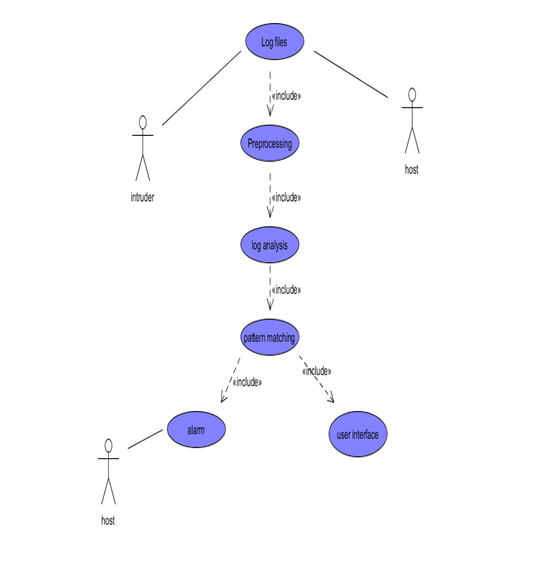
\includegraphics[width=\linewidth,height=18cm]{case.png}
  \label{fig:Use Case Diagram}
\end{figure}

\newpage
\section{Functional Model and Description}
\subsection{Data Flow Diagram}
\begin{figure}
  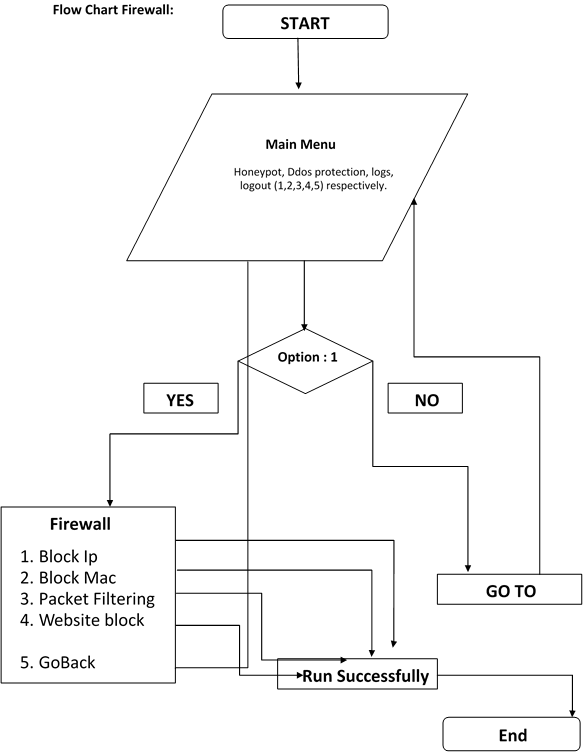
\includegraphics[width=\linewidth]{1.png}
\end{figure}
%\newpage
%\begin{figure}
 % 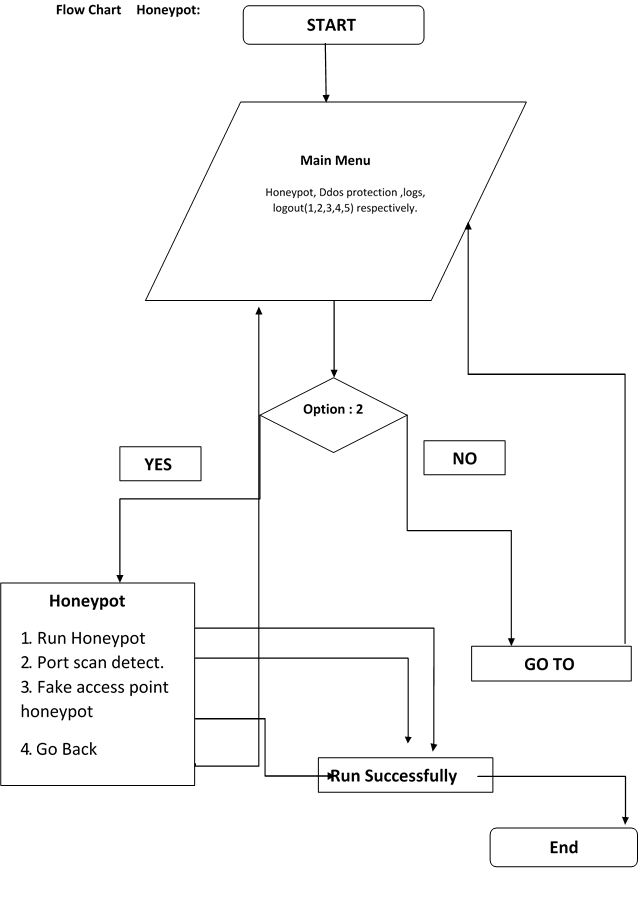
\includegraphics[width=\linewidth]{2.png}
%\end{figure}
%\newpage
%\begin{figure}
 % 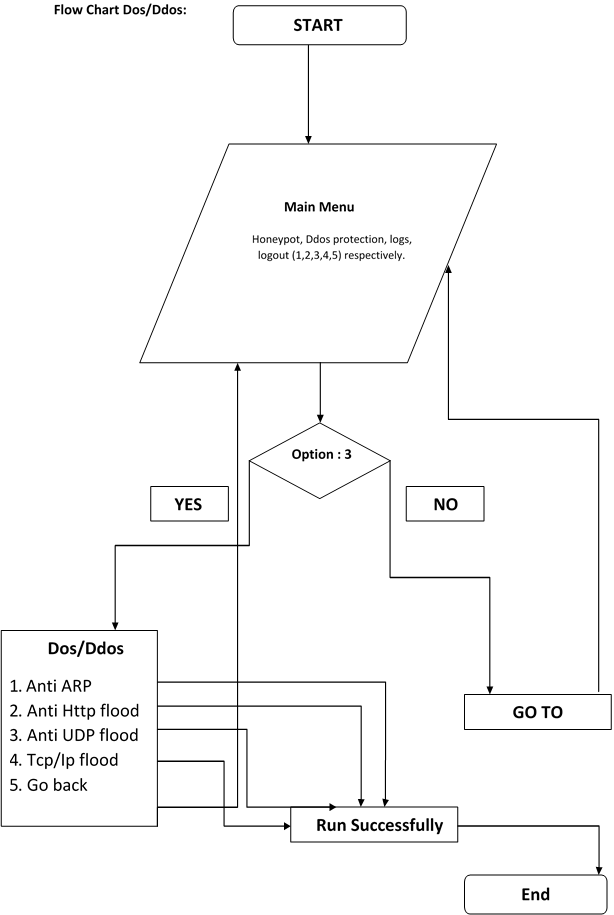
\includegraphics[width=\linewidth]{3.png}
%\end{figure}


\subsection{Activity Diagram}
Activity states represent the performance of a step within the work flow. Transitions allow transitions from one activity state to another. This is referred as completion transition. It differs from a transition in that it does not require an explicit trigger event; it is triggered by the completion of the activity that the activity state represents. Decisions for which a set of guard conditions are defined. These guard conditions control which transition of a set of alternative transitions follows once the activity has been completed. You may also use the decision icon to show where the threads merge again. Decisions and guard conditions allow you to show alternative threads in the work flow of a business use. There are actually 2 activity diagrams i.e. for admin and user.
\begin{figure}
  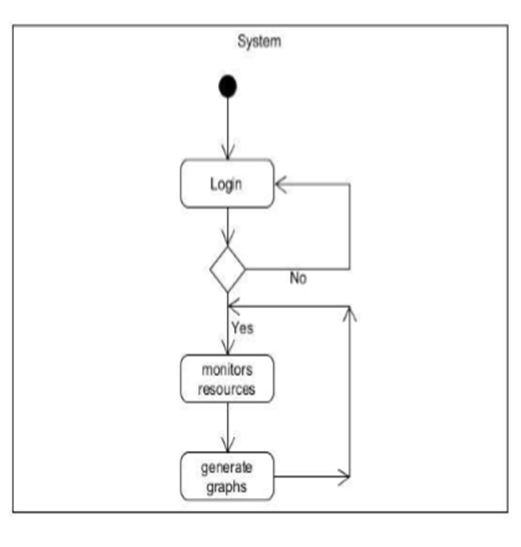
\includegraphics[width=\linewidth]{act.png}
\end{figure}

\chapter{References}
\newpage
\begin{enumerate}
\item	Ahmed Patel, Qais Qassim, Christopher Wills. A survey of intrusion detection and prevention systems, Information Management \& Computer Security Journal (2010).
\item Oludele Awodele, Sunday Idowu, Omotola Anjorin, and Vincent J. Joshua, A Multi-Layered Approach to the Design of Intelligent Intrusion Detection and Prevention System (IIDPS), Babcock University, (Volume 6, 2009).
\item	Host Intrusion Prevention Systems and Beyond, SANS Institute (2008).
\item	Intrusion Detection and Prevention In-sourced or Out-sourced, SANS Institute (2008).
\item	Mario Guimaraes, Meg Murray. Overview of Intrusion Detection and Intrusion Prevention, Information security curriculum development Conference by ACM (2008).
\item	Muhammad Awais Shibli, Sead Muftic. Intrusion Detection and Prevention System using Secure Mobile Agents,IEEE International Conference on Security \& Cryptography (2008).
\item	David Wagner, Paolo Soto. Mimicry Attacks on Host Based Intrusion Detection Systems, 9th ACM Conference on Computer and Communications Security (2002).
\item	Harley Kozushko. Intrusion Detection: Host-Based and Network-Based Intrusion Detection Systems, (2003).
\item	Lin Tan, Timothy Sherwood. A High Throughput String Matching Architecture for Intrusion Detection and Prevention, Proceedings of the 32nd Annual International Symposium on Computer Architecture (ISCA 2005).
\item	S. Mrdovic, E. Zajko. Secured Intrusion Detection System Infrastructure, University of Sarajevo/Faculty of Electrical Engineering, Sarajevo, Bosnia and Herzegovina (ICAT 2005).
\item	Yeubin Bai, Hidetsune Kobayashi. Intrusion Detection Systems: technology and Development, 17th International Conference of Advanced Information Networking and Applications, (AINA 2003).

\end{enumerate}


\end{document}